\section{Przetwornik A/C typu FLASH}

\subsection{}
Zapoznano się z budową i działaniem modułów:
\begin{itemize}
    \item Moduł komparatorów
    \item Transkoder ``Ręcznie Programowana Pamięć Stała'' (RPP-S)
    \item Transkoder ``Ręcznie Programowana Pamięć SRAM'' (RPP-SRAM)
    \item Przetwornik Cyfrowo - Analogowy
\end{itemize}

\subsection{}
Moduł komparatorów połączono z Transkoderem RPP-S.
Następnie za pomocą zasilacza laboratoryjnego podano regulowane napięcie stałe na wejście modułu komparatora.
Napięcie dobrano tak aby żadna z diod LED na module RPP-S nie była zapalona.
Z użyciem przełączników na płycie transkodera zaprogramowano układ tak aby wartość binarna na jego wyjściu odzwierciedlała ilość aktywnych diod LED.
Krok ten powtarzano każdorazowo zwiększając napięcie wyjściowe zasilacza laboratoryjnego, zwiększając tym samym ilość zapalonych diod.

\subsection{}
Po zaprogramowaniu modułu RPP-S podłączono do niego płytkę przetwornika C/A.
Następnie za pomocą generatora funkcyjnego na wejście modułu komparatorów podano napięcie sinusoidalne.
Do wyjścia przetwornika C/A podłączono oscyloskop. Zmierzone napięcie pokazano na Rys. \refeq{ca_test}, widoczna jest kwantyzacja sygnału.
\begin{figure}[H]
    \centering
    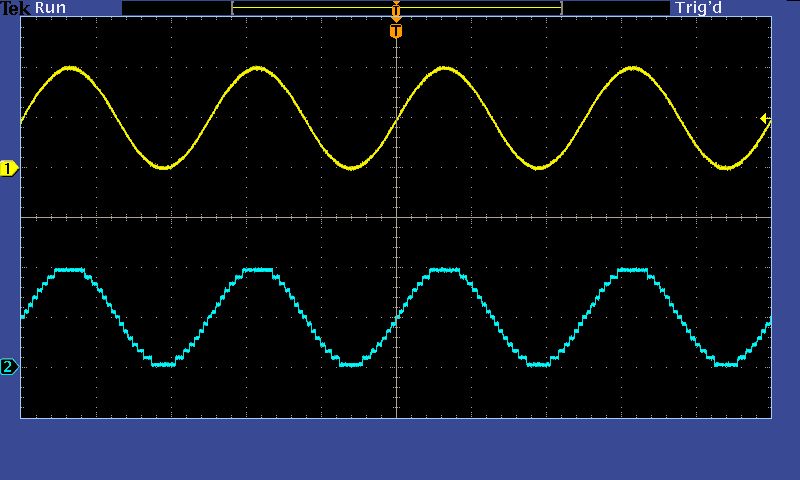
\includegraphics[width=\textwidth]{include/3/1.png}
    \caption{Na żółto: napięcie podane z generatora funkcyjnego, na niebiesko: napięcie na wyjściu przetwornika C/A}
    \label{ca_test}
\end{figure}

\subsection{}
Zmodyfikowano układ testowy zastępując transkoder RPP-S transkoderem RPP-SRAM.
Postępując analogicznie do modułu z pamięcią stałą zaprogramowano transkoder z pamięcią SRAM.
Dla każdej ilości aktywnych na module komparatorów diod LED, ustawiano odpowiadają im kombinację przełączników na płycie RPP-SRAM, a następnie zapisywano ich stan w pamięci SRAM za pomocą przycisków OE oraz WE.
Ponownie sprawdzono działanie transkodera za pomocą przetwornika C/A i oscyloskopu.